\documentclass{bredelebeamer}

%%%%%%%%%%%%%%%%%%%%%%%%%%%%%%%%%%%%%%%%%%%%%%%%

\title[Programación en MatLAB]{Introducción a la programación con MatLAB}
\subtitle{Modulo 01 - Introducción al curso}

\author{Agustín - Andrés - Gabriel - Fernando\inst{1}}
\institute[UTN.BA]
{
  \inst{1}%
  Universidad Tecnológica Nacional\\
  Facultad Regional Buenos Aires
  }

\date{2018}

\subject{Taller de programación}

\logo{

\includegraphics[scale=0.15]{images/logo.png}
}

%%%%%%%%%%%%%%%%%%%%%%%%%%%%%%%%%%%%%%%%%%%%%%%%%%%%%%%%%%%%%%%%%%%%%
\begin{document}

\begin{frame}
  \titlepage 
\end{frame}

%%%%%%%%%%%%%%%%%%%%%%%%%%%%%%%%%%%%%%%%%%%%%%%%%%%%%%%%%%%%%%%%%%%%%

% Sección de introducción al taller

%%%%%%%%%%%%%%%%%%%%%%%%%%%%%%%%%%%%%%%%%%%%%%%%%%%%%%%%%%%%%%%%%%%%%
\section{Introducción al taller}

\begin{frame}{Introducción al taller}
\textbf{Premisas iniciales:}
\begin{columns}
\begin{column}{0.5\textwidth}
\begin{itemize}
\item Duración: 5 clases teóricas/prácticas
\item Destinatario: Alumnos de ingeniería
\item Taller a cargo de
\begin{itemize}
\item Agustín Ortiz
\item Andrés Hojnadel
\item Gabriel Maroli
\item Fernando Pose
\end{itemize}
\end{itemize}
\begin{center}
\textit{Se entregarán certificados de asistencia a quienes asistan a ambos encuentros.
}\end{center}
\end{column}
\begin{column}{0.3\textwidth}

\includegraphics[scale=0.3]{images/matlab.jpg}
\end{column}
\end{columns}
\end{frame}

\begin{frame}{Introducción al taller}
\textbf{Qué resultará de este taller?}\\
\begin{itemize}
\item Obtendrán los conocimientos básicos teóricos y prácticos que les permitirán trabajar en Matlab y Simulink
\item Podrán verificar e implementar soluciones simples a distintos problemas
\item Estarán familiarizados con las funciones básicas que ofrece Matlab y Simulink
\end{itemize}
\end{frame}

%%%%%%%%%%%%%%%%%%%%%%%%%%%%%%%%%%%%%%%%%%%%%%%%%%%%%%%%%%%%%%%%%%%%%

% Sección matlab

%%%%%%%%%%%%%%%%%%%%%%%%%%%%%%%%%%%%%%%%%%%%%%%%%%%%%%%%%%%%%%%%%%%%%

\section{MatLAB}

\begin{frame}{Qué es Matlab?}
\begin{block}{Matlab es..}
Una sofisticada herramienta de computación disponible para resolver problemas de matemática, tales como Maple, Mathematica y MathCad.
\end{block}
\end{frame}

\begin{frame}{Qué es Matlab?}
\begin{block}{Matlab es..}
Una sofisticada herramienta de computación disponible para resolver problemas de matemática, tales como Maple, Mathematica y MathCad.
\end{block}
\Large Además \normalsize
\begin{itemize}
\item Un lenguaje de programación
\item Un lenguaje de programación interpretado
\item Un lenguaje de programación interactivo
\end{itemize}
\end{frame}

\begin{frame}{Lenguaje interpretado}
\begin{itemize}
\item Es como un actor que hace todo lo que dice un guión
\item Muy parecido a una calculadora
\item Es interactivo
\end{itemize}
\begin{center}
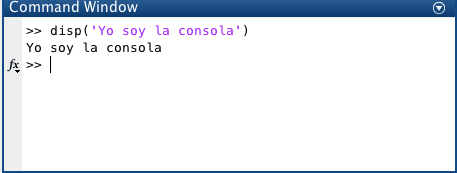
\includegraphics[scale=0.5]{images/consola.png}
\end{center}
\end{frame}

\begin{frame}{Qué no es Matlab?}
\begin{itemize}
\item Una hoja de cálculo
\item Un programa de cálculo simbólico
\item La solución a todos nuestros problemas
\end{itemize}
\end{frame}

\begin{frame}{Posibles campos de aplicación}
\begin{center}

\includegraphics[scale=0.4]{images/img40.png}\\
\end{center}
\begin{center}
\textit{"La computadora va a pensar por nosotros"}
\end{center}
\end{frame}

\begin{frame}{Posibles campos de aplicación}
\begin{columns}
\begin{column}{0.5\textwidth}
\begin{center}
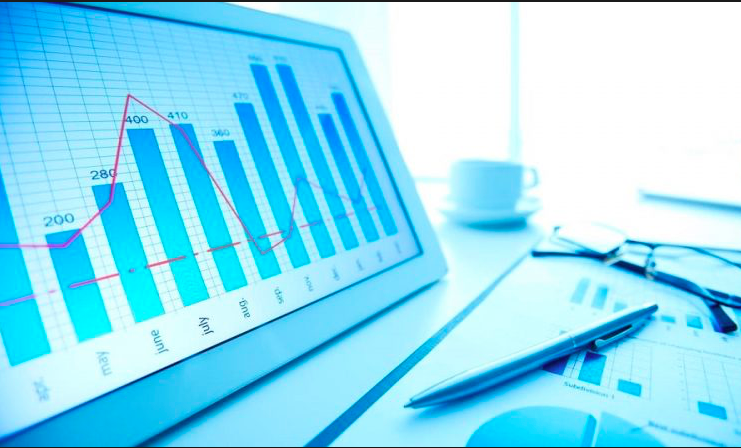
\includegraphics[scale=0.2]{images/ap1.png}\\
\end{center}
\end{column}
\begin{column}{0.3\textwidth}
\begin{center}
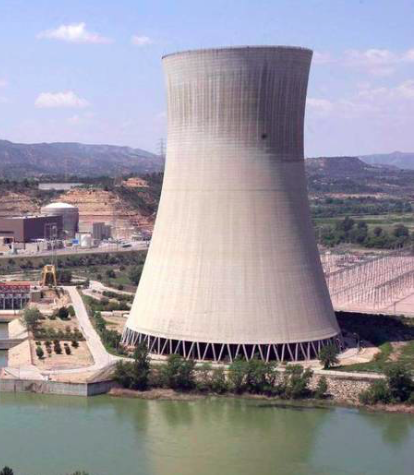
\includegraphics[scale=0.2]{images/ap2.png}\\
\end{center}
\end{column}
\begin{column}{0.3\textwidth}
\begin{center}
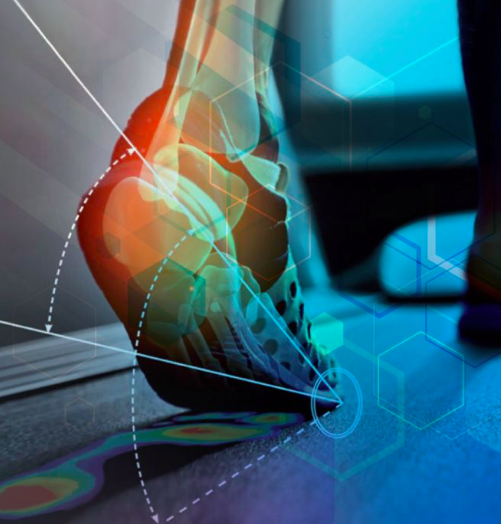
\includegraphics[scale=0.19]{images/ap3.png}\\
\end{center}
\end{column}
\end{columns}
\end{frame}

\begin{frame}{Posibles campos de aplicación}
\begin{columns}
\begin{column}{0.5\textwidth}
\begin{center}
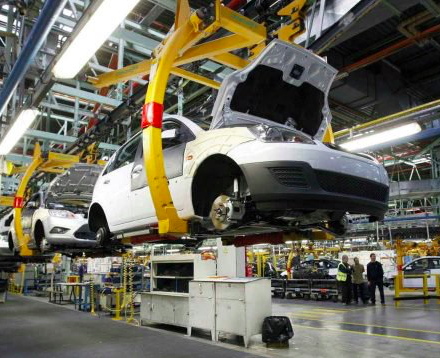
\includegraphics[scale=0.3]{images/ap4.png}
\end{center}
\end{column}
\begin{column}{0.3\textwidth}
\begin{center}
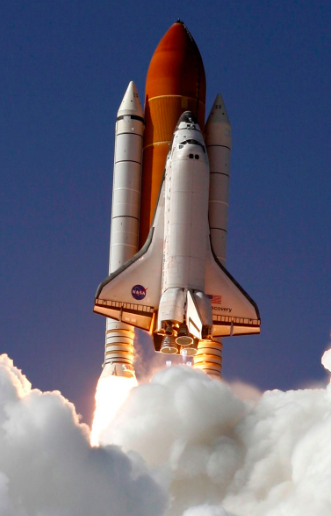
\includegraphics[scale=0.18]{images/ap5.png}
\end{center}
\end{column}
\begin{column}{0.23\textwidth}
\begin{center}
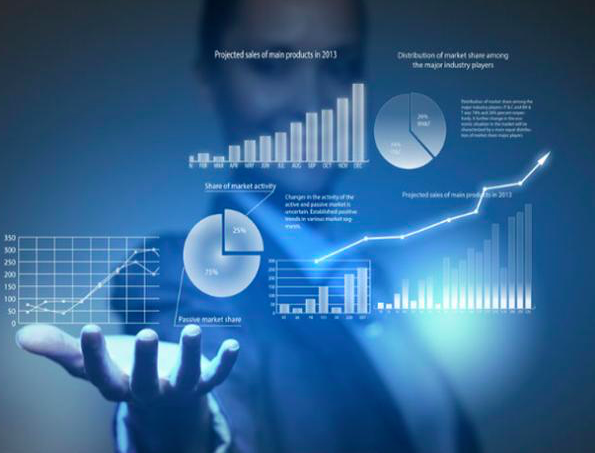
\includegraphics[scale=0.18]{images/ap6.png}
\end{center}
\end{column}
\end{columns}
\end{frame}

%%%%%%%%%%%%%%%%%%%%%%%%%%%%%%%%%%%%%%%%%%%%%%%%%%%%%%%%%%%%%%%%%%%%%

% Sección taller intro

%%%%%%%%%%%%%%%%%%%%%%%%%%%%%%%%%%%%%%%%%%%%%%%%%%%%%%%%%%%%%%%%%%%%%

\section{Intro}

\begin{frame}{Temario}
\begin{center}
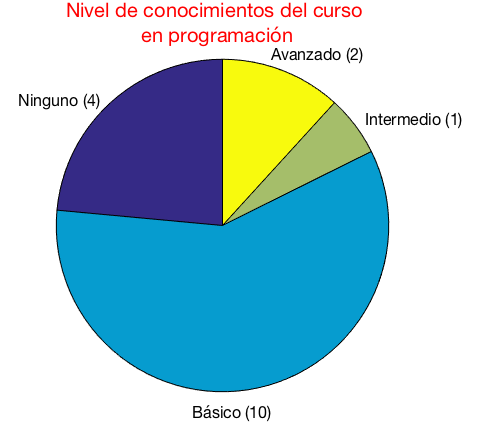
\includegraphics[scale=0.35]{images/estadisticas.png}
\end{center}
\end{frame}

\begin{frame}{Temario}
El temario se divide en los siguientes \textbf{5 bloques}:
\begin{columns}
\begin{column}{0.5\textwidth}
\begin{itemize}
\item \textbf{Módulo 1:} Ambiente de Matlab 
\item \textbf{Módulo 2:} Fundamentos de Matlab 
\item \textbf{Módulo 3:} Estructuras de control
\item \textbf{Módulo 4:} Cálculo simólico
\end{itemize}
\end{column}
\begin{column}{0.3\textwidth}
\begin{center}

\includegraphics[scale=0.25]{images/matlab.jpg}
\end{center}
\end{column}
\end{columns}
\begin{columns}
\begin{column}{0.3\textwidth}
\begin{center}

\includegraphics[scale=0.3]{images/img41.png}
\end{center}
\end{column}
\begin{column}{0.5\textwidth}
\begin{itemize}
\item \textbf{Módulo 5:} Introducción a Simulink
\end{itemize}
\end{column}
\end{columns}
\end{frame}

\begin{frame}{Introducción al taller}
\begin{large}
\begin{center}
"No escribí el ejemplos porque era demasiado sencillo"
\end{center}
\end{large}
\end{frame}

\begin{frame}{Introducción al taller}
\begin{large}
\begin{center}

\includegraphics[scale=0.27]{images/img42.jpg}
\end{center}
\end{large}
\end{frame}

\begin{frame}{Introducción al taller}
\begin{Huge}
\begin{center}

\includegraphics[scale=0.1]{images/exclamacion.png}
\\No se aprende a programar leyendo \\Se aprende sentándose y programando 
\end{center}
\end{Huge}
\end{frame}

\begin{frame}{Algunas mentiras}
\begin{columns}
\begin{column}{0.5\textwidth}
\begin{itemize}
\item Para ser ingeniero no es necesario saber programar
\item Programar es difícil
\item Programar bien es fácil
\item Los ingenieros programan bien
\item En la vida basta un solo lenguaje de programación mientras se domine.
\end{itemize}
\end{column}
\begin{column}{0.23\textwidth}
\begin{center}

\includegraphics[scale=0.18]{images/img43.png}
\end{center}
\end{column}
\end{columns}
\end{frame}

%%%%%%%%%%%%%%%%%%%%%%%%%%%%%%%%%%%%%%%%%%%%%%%%%%%%%%%%%%%%%%%%%%%%%

% Sección de bibliografía

%%%%%%%%%%%%%%%%%%%%%%%%%%%%%%%%%%%%%%%%%%%%%%%%%%%%%%%%%%%%%%%%%%%%%

\section{Bibliografia}

\begin{frame}{Bibliografía}
\begin{columns}
\begin{column}{0.5\textwidth}
\begin{center}

\includegraphics[scale=0.4]{images/biblio1.png}
\end{center}
\end{column}
\begin{column}{0.5\textwidth}
\begin{center}
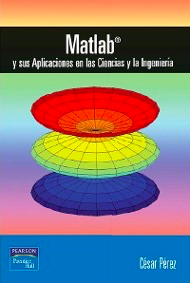
\includegraphics[scale=0.5]{images/biblio2.png}
\end{center}
\end{column}
\end{columns}

Nota: la web de \textbf{MathWorks} siempre es una excelente opción para dudas puntuales.
\end{frame}

\end{document}
